\appendix
%%%%%%%%% ANNEX A
\chapter{Acr\'onimos}
\label{an:Annex_A_Acronimos}
Acrónimos usados en el presente trabajo de investigación:
\begin{acronym}[ABCDEFGHIJK]
%A
\acro{TFC2}{Trabajo de Fin de Carrera 2}
\acro{TDAH}{Trastorno de Déficit de Atención e Hiperactividad}
\acro{BF}{Baja frecuencia}
\acro{AF}{Alta frecuencia}
\acro{SW}{Software}
\acro{CoS}{Concepto de solución}
%\ac{API}
%D
%\acro{DC}{\textit{Direct Current}} %\ac{DC}
%E
%\acro{ETAP}{\textit{Electrical Transient and Analysis Program}}
%F
%\acro{FEM}{Fuerza contraelectromotriz}
%\acro{FPGA}{\textit{Field-Programmable Gate Array}}
%G
%\acro{GUI}{\textit{Graphical User Interface}}
%H
%\acro{HW}{Hardware} %\ac{HW}
%M
%\acro{MEE}{Modelo de Espacio de Estados}
%\acro{MIMO}{\textit{Multiple Input Multiple Output}}
%\acro{MCB}{\textit{Motor Control Blockset}}
%\acro{MQTT}{\textit{Message Queuing Telemetry Transport}}
%N
%\acro{TRL}{\textit{Technological Readiness %Level}}
%P
%\acro{PC}{\textit{Personal Computer}}
%\acro{PCB}{\textit{Printed Circuit Board}}
%\acro{PUCP}{Pontificia Universidad Católica %del Perú}

%S
%acro{SW}{Software}
%\acro{SWA}{Software A}
%\acro{SWB}{Software B}
%\acro{SISO}{\textit{Single Input Single Output}}
%\acro{SBC}{\textit{Single Board Computer}}
\end{acronym}    
\cleardoublepage 
%%%%%%%%% ANNEX B
\chapter{Lista de requerimientos}
\label{an:Annex_B_TablaVariables}
\begin{itemize}
\item Precios preliminares del concepto de solución 1: 
% \usepackage{array}
% \usepackage{multirow}
% \usepackage{ragged2e}
% \usepackage{colortbl}
% \usepackage{hhline}


\begin{table}[H]
\centering
\arrayrulecolor{black}
\begin{tabular}{|>{\hspace{0pt}}m{0.5\linewidth}|>{\centering\hspace{0pt}}m{0.117\linewidth}|>{\centering\hspace{0pt}}m{0.163\linewidth}|>{\hspace{0pt}}m{0.069\linewidth}|} 
\hline
\multicolumn{1}{|>{\centering\hspace{0pt}}m{0.5\linewidth}|}{\multirow{2}{*}{\centering Componente}} & \multicolumn{2}{c|}{Concepto Solución1} & {\cellcolor[rgb]{0.753,0.753,0.753}} \\ 
\cline{2-3}
\multicolumn{1}{|>{\centering\hspace{0pt}}m{0.5\linewidth}|}{} & \centering Unidad & \centering Por mayor & \multirow{-2}{*}{\cellcolor[rgb]{0.753,0.753,0.753}} \\ 
\hline
Motor de Vibración : 316040001 & \$1.20 & \$1.20 & \href{https://www.digikey.com/en/products/detail/seeed-technology-co-ltd/316040001/5487672}{Link} \\ 
\hline
Microcontrolador: NRF5340 & \$7.68 & \$6.54 & \href{https://www.digikey.com/en/products/detail/nordic-semiconductor-asa/NRF5340-QKAA-R/13559661}{Link} \\ 
\hline
Bateria recargable: GRP1254G1 & \$6.99 & \$6.99 & \href{https://www.digikey.com/en/products/detail/grepow-inc/GRP1254G1-3C-3-85V-75mAh/25603168}{Link} \\ 
\hline
Interruptor deslizante: MSS-102559-14A-D & \$0.90 & \$0.53 & \href{https://www.digikey.com/en/products/detail/same-sky-formerly-cui-devices/MSS-102559-14A-D/13978983}{Link} \\ 
\hline
Regulador Buck: TPS62840DLCR & \$1.80 & \$0.93 & \href{https://www.digikey.com/en/products/detail/texas-instruments/TPS62840DLCR/10445071}{Link} \\ 
\hline
Sensor: MAX30102EFD & \$12.04 & \$8.00 & \href{https://www.digikey.com/en/products/detail/analog-devices-inc-maxim-integrated/MAX30102EFD-T/6188734}{Link} \\ 
\hhline{|====|}
Total & \$30.61 & \$24.19 & {\cellcolor[rgb]{0.753,0.753,0.753}} \\
\hline
\end{tabular}
\end{table}


\item Precios preliminares del concepto de solución 2:


\begin{table}[H]
\centering
\arrayrulecolor{black}
\begin{tabular}{|>{\hspace{0pt}}m{0.5\linewidth}|>{\centering\hspace{0pt}}m{0.115\linewidth}|>{\centering\hspace{0pt}}m{0.163\linewidth}|>{\hspace{0pt}}m{0.069\linewidth}|} 
\hline
\multicolumn{1}{|>{\centering\hspace{0pt}}m{0.5\linewidth}|}{\multirow{2}{0.588\linewidth}{\hspace{0pt}\centering{}Componente}} & \multicolumn{2}{>{\centering\hspace{0pt}}m{0.278\linewidth}|}{Concepto Solución 2} & {\cellcolor[rgb]{0.753,0.753,0.753}}                                              \\ 
\hhline{|~-->{\arrayrulecolor[rgb]{0,0,0}}->{\arrayrulecolor{black}}|}
\multicolumn{1}{|>{\centering\hspace{0pt}}m{0.5\linewidth}|}{}                                                                  & Unidad  & Por mayor                                                                & \multirow{-2}{0.065\linewidth}{\hspace{0pt}{\cellcolor[rgb]{0.753,0.753,0.753}}}  \\ 
\hline
Motor de Vibración : 316040001                                                                                                    & \$1.20  & \$1.20                                                                   & \href{https://www.digikey.com/en/products/detail/seeed-technology-co-ltd/316040001/5487672}{Link}                                                                              \\ 
\hline
Microcontrolador: DA14531                                                                                                         & \$2.04  & \$1.33                                                                   & \href{https://www.digikey.com/en/products/detail/renesas-electronics-corporation/DA14531-00000OG2/10474922}{Link}                                                                              \\ 
\hline
Bateria recargable: RJD2048                                                                                                       & \$10.70 & \$7.85                                                                   & \href{https://www.digikey.com/en/products/detail/cornell-dubilier-knowles/RJD2048/6159136}{Link}                                                                              \\ 
\hline
Interruptor tipo boton:  PTS810SJK250SMTR                                                                                         & \$0.51  & \$0.30                                                                   & \href{https://www.digikey.es/es/products/detail/c-k/PTS810SJK250SMTR-LFS/4176611?srsltid=AfmBOoqM8RznWfZIkPvuGBnjfKT_Ri67wlrvbd_l-FHUMYyJ-5bTSpv4}{Link}                                                                              \\ 
\hline
Regulador Buck: TPS62840DLCR                                                                                                      & \$1.80  & \$0.93                                                                   & \href{https://www.digikey.com/en/products/detail/texas-instruments/TPS62840DLCR/10445071}{Link}                                                                              \\ 
\hline
Sensor: MAX30102EFD                                                                                                               & \$12.04 & \$8.00                                                                   & \href{https://www.digikey.com/en/products/detail/analog-devices-inc-maxim-integrated/MAX30102EFD-T/6188734}{Link}                                                                              \\ 
\hhline{|====|}
Total                                                                                                                             & \$28.29 & \$19.61                                                                  & {\cellcolor[rgb]{0.753,0.753,0.753}}                                              \\
\hline
\end{tabular}
\end{table}




\item Precios preliminares del concepto de solución 3: 

\begin{table}[H]
\centering
\arrayrulecolor{black}
\begin{tabular}{|>{\hspace{0pt}}m{0.5\linewidth}|>{\centering\hspace{0pt}}m{0.119\linewidth}|>{\centering\hspace{0pt}}m{0.167\linewidth}|>{\hspace{0pt}}m{0.067\linewidth}|} 
\hline
\multicolumn{1}{|>{\centering\hspace{0pt}}m{0.5\linewidth}|}{\multirow{2}{0.579\linewidth}{\hspace{0pt}\centering{}Componente}} & \multicolumn{2}{>{\centering\hspace{0pt}}m{0.286\linewidth}|}{Concepto Solución 3} & {\cellcolor[rgb]{0.753,0.753,0.753}}                                              \\ 
\hhline{|~-->{\arrayrulecolor[rgb]{0.753,0.753,0.753}}->{\arrayrulecolor{black}}|}
\multicolumn{1}{|>{\centering\hspace{0pt}}m{0.5\linewidth}|}{}                                                                  & Unidad  & Por mayor                                                                & \multirow{-2}{0.067\linewidth}{\hspace{0pt}{\cellcolor[rgb]{0.753,0.753,0.753}}}  \\ 
\hline
Zumbador piezoelectrico: GT-0950RP3                                                                                               & \$1.73  & \$0.93                                                                   & \href{https://www.digikey.com/en/products/detail/visaton-gmbh-co-kg/MB-12-5-V/10650231}{Link}                                                                              \\ 
\hline
Microcontrolador: ESP32-C3                                                                                                        & \$1.07  & \$1.00                                                                   & \href{https://www.digikey.com/en/products/detail/espressif-systems/ESP32-C3/14115579}{Link}                                                                              \\ 
\hline
Bateria recargable: RTU-NiMH                                                                                                      & \$6.50  & \$5.50                                                                   & \href{https://www.digikey.com/en/products/detail/pkcell/RTU-NiMH-9V250-1B/22152886}{Link}                                                                              \\ 
\hline
Interruptor deslizante: MSS-102559-14A-D                                                                                          & \$0.90  & \$0.53                                                                   & \href{https://www.digikey.com/en/products/detail/same-sky-formerly-cui-devices/MSS-102559-14A-D/13978983}{Link}                                                                              \\ 
\hline
Regulador Buck: TPS62840DLCR                                                                                                      & \$1.80  & \$0.93                                                                   & \href{https://www.digikey.com/en/products/detail/texas-instruments/TPS62840DLCR/10445071}{Link}                                                                              \\ 
\hline
Sensor: LIS2DH12TR                                                                                                                & \$1.43  & \$0.90                                                                   & \href{https://www.digikey.com/en/products/detail/stmicroelectronics/LIS2DH12TR/4899892?s=N4IgTCBcDaIDIEkDKYAiAJAjGABCAugL5A}{Link}                                                                              \\ 
\hhline{|====|}
Total                                                                                                                             & \$13.43 & \$9.79                                                                   & {\cellcolor[rgb]{0.753,0.753,0.753}}                                              \\
\hline
\end{tabular}
\end{table}

\end{itemize}
%\begin{longtblr}[
  label = {tab:Annex_B_requerimientos},
  caption = {Lista de Requerimientos del asistente},
]{
  width = \linewidth,
  colspec =  {Q[c,m]Q[l,m]},
  column{1}={0.1\textwidth},
  column{2}={0.6\textwidth},
  row{1} = {c},
  row{3} = {c},
  row{8} = {c},
  row{11} = {c},
  row{16} = {c},
  row{19} = {c},
  row{23} = {c},
  row{27} = {c},
  row{30} = {c},
  row{32} = {c},
  row{35} = {c},
  cell{1}{1} = {c=2}{0.94\linewidth},
  cell{2}{1} = {c},
  cell{3}{1} = {c=2}{0.94\linewidth},
  cell{4}{1} = {c},
  cell{5}{1} = {c},
  cell{6}{1} = {c},
  cell{7}{1} = {c},
  cell{8}{1} = {c=2}{0.94\linewidth},
  cell{9}{1} = {c},
  cell{10}{1} = {c},
  cell{11}{1} = {c=2}{0.94\linewidth},
  cell{12}{1} = {c},
  cell{13}{1} = {c},
  cell{14}{1} = {c},
  cell{15}{1} = {c},
  cell{16}{1} = {c=2}{0.94\linewidth},
  cell{17}{1} = {c},
  cell{18}{1} = {c},
  cell{19}{1} = {c=2}{0.94\linewidth},
  cell{20}{1} = {c},
  cell{21}{1} = {c},
  cell{22}{1} = {c},
  cell{23}{1} = {c=2}{0.94\linewidth},
  cell{24}{1} = {c},
  cell{25}{1} = {c},
  cell{26}{1} = {c},
  cell{27}{1} = {c=2}{0.94\linewidth},
  cell{28}{1} = {c},
  cell{29}{1} = {c},
  cell{30}{1} = {c=2}{0.94\linewidth},
  cell{31}{1} = {c},
  cell{32}{1} = {c=2}{0.94\linewidth},
  cell{33}{1} = {c},
  cell{34}{1} = {c},
  cell{35}{1} = {c=2}{0.94\linewidth},
  cell{36}{1} = {c},
  hlines,
  vlines,
  hline{1,37} = {-}{0.08em},
}
Lista de Requerimientos &                                                                                                                           \\
D/E                     & Descripción                                                                                                               \\
Funcion principal       &                                                                                                                           \\
E                       & Detectar indicadores fisiológicos de distracción del usuario                                                              \\
E                       & Emitir retroalimentación inmediata al detectar distracción por parte del usuario a través de vibraciones                  \\
E                       & Permitir al usuario establecer la duración de su sesión de estudio                                                        \\
D                       & Ofrecer ejercicios breves de respiración guiada mediante vibración rítmica                                                \\
Geometría y ergonomía   &                                                                                                                           \\
E                       & Diseño no invasivo para el usuario                                                                                        \\
E                       & Materiales hipoalergénicos y adecuados para estar en contacto con la piel                                                 \\
Energía                 &                                                                                                                           \\
E                       & El asistente debe contar con autonomía energética                                                                         \\
E                       & El asistente debe ser capaz de poder funcionar de manera continua entre 4 y 6 horas, abarcando sesiones largas de estudio \\
E                       & Los componentes electrónicos deben de ser de bajo consumo para optimizar la duración de la batería                        \\
D                       & El asistente debe  contar con un modo de reposo o bajo consumo cuando no este en uso activo (sesión de estudio)           \\
Seguridad               &                                                                                                                           \\
E                       & Resistencia a golpes, agua y polvo grado IP67                                                                             \\
E                       & Las retroalimentaciones no deben generar incomodidad                                                                      \\
Interfaz                &                                                                                                                           \\
E                       & Interfaz amigable para que el usuario pueda interactuar con facilidad                                                     \\
E                       & Permite configurar sesiones y  consultar historial de concentración, a través de procentajes y estadística                \\
D                       & Interfaz personalizable para que el usuario la modifique de acuerdo a sus necesidades                                     \\
Comunicaciones          &                                                                                                                           \\
E                       & Comunicación con smartphones vía Bluetooth Low Energy 5.0                                                                 \\
D                       & Retardo máximo de 2 segundos de sincronización                                                                            \\
D                       & Conexión con PC mediante cable USB-C                                                                                      \\
Montaje y mantenimiento &                                                                                                                           \\
E                       & El ensamblaje del asistente debe permitir reemplazo de batería o sensores                                                 \\
E                       & Partes internas aseguradas contra el movimiento para evitar daños leves                                                   \\
Software                &                                                                                                                           \\
E                       & El software del dispositivo debe cumplir con estándares de codificación seguros y confiables, como el estándar MISRA      \\
Procesamiento           &                                                                                                                           \\
E                       & El procesamiento básico deberá realizarse localmente, sin depender de algún aplicativo                                    \\
D                       & El asistente debe almacenar datos localmente en caso de pérdida de conexión                                               \\
Costos                  &                                                                                                                           \\
E                       & El diseño debe priorizar componentes de bajo consumo y bajo costo sin comprometer precisión biométrica         
\end{longtblr}




\cleardoublepage
%%%%%%%%% ANNEX C



\chapter{Estructura de Funciones}
\label{an:Annex_estrucutra}
Con el fin de preservar la legibilidad del diagrama, la estructura de funciones se presenta en la página siguiente en tamaño A3. De esta manera se garantiza que los elementos y conexiones puedan visualizarse con claridad, sin pérdida de detalle.

% Forzar salto de página: el capítulo en A4, la figura en la siguiente
\clearpage 

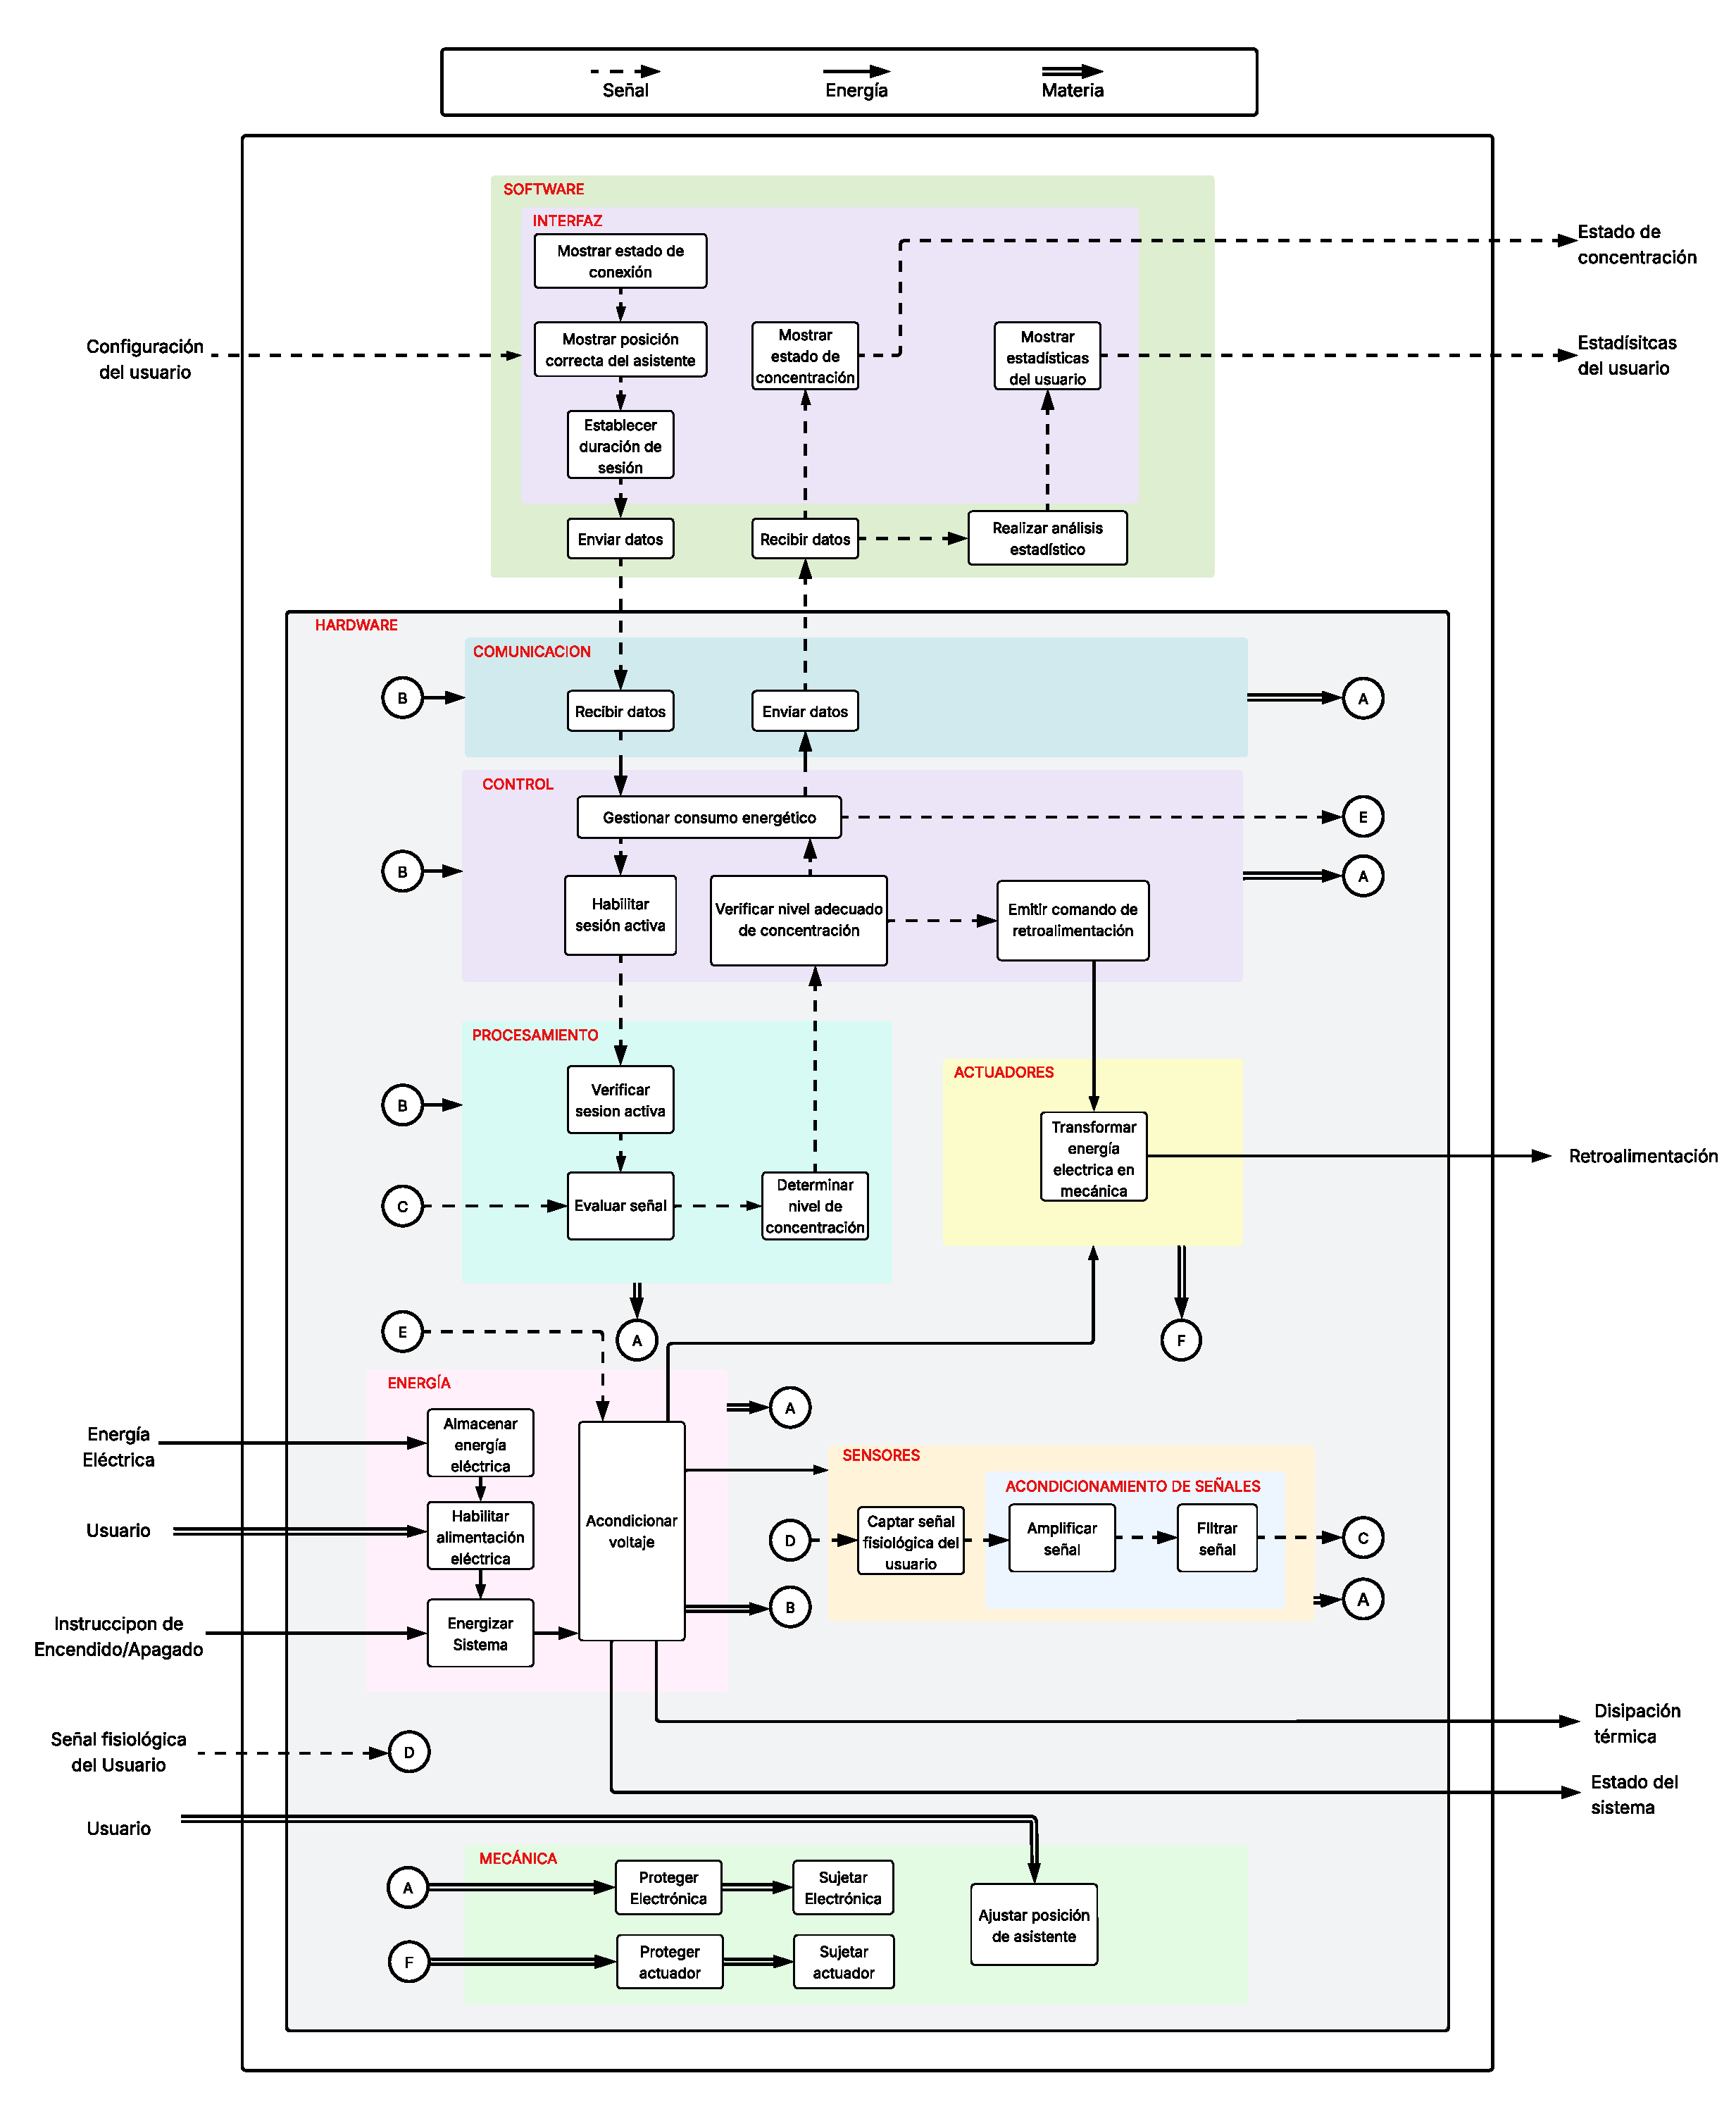
\includepdf[
  pages=-,
  pagecommand={\thispagestyle{empty}}, % sin título ni número
  fitpaper=true,
  paper=a3paper
]{CHPTRS/CH03_DICON/fig_cap3/Estructura de funciones tesis.pdf}



\chapter{Listas de precios preliminar para el análisis económico}
\label{an:Annex_D_precios_preliminares}

Para realizar las siguientes tablas preliminares de cotización se utilizó la plataforma \textit{Digikey} en el mes de junio del año 2025. Asimismo, se consideró que los precios por mayor a partir de 1000 unidades. \\
\begin{itemize}
\item Precios preliminares del concepto de solución 1: 
% \usepackage{array}
% \usepackage{multirow}
% \usepackage{ragged2e}
% \usepackage{colortbl}
% \usepackage{hhline}


\begin{table}[H]
\centering
\arrayrulecolor{black}
\begin{tabular}{|p{0.55\linewidth}|c|c|} 
\hline
\multicolumn{1}{|c|}{\multirow{2}{*}{Componente}} & \multicolumn{2}{c|}{Concepto Solución1} \\ 
\cline{2-3}
\multicolumn{1}{|c|}{} & Unidad & Por mayor \\ 
\hline
Motor de Vibración: \href{https://www.digikey.com/en/products/detail/seeed-technology-co-ltd/316040001/5487672}{316040001} & \$1.20 & \$1.20 \\ 
\hline
Microcontrolador: \href{https://www.digikey.com/en/products/detail/nordic-semiconductor-asa/NRF5340-QKAA-R/13559661}{NRF5340} & \$7.68 & \$6.54 \\ 
\hline
Batería recargable: \href{https://www.digikey.com/en/products/detail/grepow-inc/GRP1254G1-3C-3-85V-75mAh/25603168}{GRP1254G1} & \$6.99 & \$6.99 \\ 
\hline
Interruptor deslizante: \href{https://www.digikey.com/en/products/detail/same-sky-formerly-cui-devices/MSS-102559-14A-D/13978983}{MSS-102559-14A-D} & \$0.90 & \$0.53 \\ 
\hline
Regulador Buck: \href{https://www.digikey.com/en/products/detail/texas-instruments/TPS62840DLCR/10445071}{TPS62840DLCR} & \$1.80 & \$0.93 \\ 
\hline
Sensor: \href{https://www.digikey.com/en/products/detail/analog-devices-inc-maxim-integrated/MAX30102EFD-T/6188734}{MAX30102EFD} & \$12.04 & \$8.00 \\ 
\hhline{|===|}
Total & \$30.61 & \$24.19 \\
\hline
\end{tabular}
\end{table}


\item Precios preliminares del concepto de solución 2:


\begin{table}[H]
\centering
\arrayrulecolor{black}
\begin{tabular}{|p{0.55\linewidth}|c|c|} 
\hline
\multicolumn{1}{|c|}{\multirow{2}{*}{Componente}} & \multicolumn{2}{c|}{Concepto Solución 2} \\ 
\cline{2-3}
\multicolumn{1}{|c|}{} & Unidad & Por mayor \\ 
\hline
Motor de Vibración: \href{https://www.digikey.com/en/products/detail/seeed-technology-co-ltd/316040001/5487672}{316040001} & \$1.20 & \$1.20 \\ 
\hline
Microcontrolador: \href{https://www.digikey.com/en/products/detail/renesas-electronics-corporation/DA14531-00000OG2/10474922}{DA14531} & \$2.04 & \$1.33 \\ 
\hline
Batería recargable: \href{https://www.digikey.com/en/products/detail/cornell-dubilier-knowles/RJD2048/6159136}{RJD2048} & \$10.70 & \$7.85 \\ 
\hline
Interruptor tipo botón: \href{https://www.digikey.es/es/products/detail/c-k/PTS810SJK250SMTR-LFS/4176611?srsltid=AfmBOoqM8RznWfZIkPvuGBnjfKT_Ri67wlrvbd_l-FHUMYyJ-5bTSpv4}{PTS810SJK250SMTR} & \$0.51 & \$0.30 \\ 
\hline
Regulador Buck: \href{https://www.digikey.com/en/products/detail/texas-instruments/TPS62840DLCR/10445071}{TPS62840DLCR} & \$1.80 & \$0.93 \\ 
\hline
Sensor: \href{https://www.digikey.com/en/products/detail/analog-devices-inc-maxim-integrated/MAX30102EFD-T/6188734}{MAX30102EFD} & \$12.04 & \$8.00 \\ 
\hhline{|===|}
Total & \$28.29 & \$19.61 \\
\hline
\end{tabular}
\end{table}


\clearpage


\item Precios preliminares del concepto de solución 3: 

\begin{table}[H]
\centering
\arrayrulecolor{black}
\begin{tabular}{|p{0.55\linewidth}|c|c|} 
\hline
\multicolumn{1}{|c|}{\multirow{2}{*}{Componente}} & \multicolumn{2}{c|}{Concepto Solución 3} \\ 
\cline{2-3}
\multicolumn{1}{|c|}{} & Unidad & Por mayor \\ 
\hline
Zumbador piezoeléctrico: \href{https://www.digikey.com/en/products/detail/visaton-gmbh-co-kg/MB-12-5-V/10650231}{MB-12-5-V} & \$1.73 & \$0.93 \\ 
\hline
Microcontrolador: \href{https://www.digikey.com/en/products/detail/espressif-systems/ESP32-C3/14115579}{ESP32-C3} & \$1.07 & \$1.00 \\ 
\hline
Batería recargable: \href{https://www.digikey.com/en/products/detail/pkcell/RTU-NiMH-9V250-1B/22152886}{RTU-NiMH} & \$6.50 & \$5.50 \\ 
\hline
Interruptor deslizante: \href{https://www.digikey.com/en/products/detail/same-sky-formerly-cui-devices/MSS-102559-14A-D/13978983}{MSS-102559-14A-D} & \$0.90 & \$0.53 \\ 
\hline
Regulador Buck: \href{https://www.digikey.com/en/products/detail/texas-instruments/TPS62840DLCR/10445071}{TPS62840DLCR} & \$1.80 & \$0.93 \\ 
\hline
Sensor: \href{https://www.digikey.com/en/products/detail/stmicroelectronics/LIS2DH12TR/4899892?s=N4IgTCBcDaIDIEkDKYAiAJAjGABCAugL5A}{LIS2DH12TR} & \$1.43 & \$0.90 \\ 
\hhline{|===|}
Total & \$13.43 & \$9.79 \\
\hline
\end{tabular}
\end{table}


\end{itemize}
%\begin{longtblr}[
  label = {tab:Annex_B_requerimientos},
  caption = {Lista de Requerimientos del asistente},
]{
  width = \linewidth,
  colspec =  {Q[c,m]Q[l,m]},
  column{1}={0.1\textwidth},
  column{2}={0.6\textwidth},
  row{1} = {c},
  row{3} = {c},
  row{8} = {c},
  row{11} = {c},
  row{16} = {c},
  row{19} = {c},
  row{23} = {c},
  row{27} = {c},
  row{30} = {c},
  row{32} = {c},
  row{35} = {c},
  cell{1}{1} = {c=2}{0.94\linewidth},
  cell{2}{1} = {c},
  cell{3}{1} = {c=2}{0.94\linewidth},
  cell{4}{1} = {c},
  cell{5}{1} = {c},
  cell{6}{1} = {c},
  cell{7}{1} = {c},
  cell{8}{1} = {c=2}{0.94\linewidth},
  cell{9}{1} = {c},
  cell{10}{1} = {c},
  cell{11}{1} = {c=2}{0.94\linewidth},
  cell{12}{1} = {c},
  cell{13}{1} = {c},
  cell{14}{1} = {c},
  cell{15}{1} = {c},
  cell{16}{1} = {c=2}{0.94\linewidth},
  cell{17}{1} = {c},
  cell{18}{1} = {c},
  cell{19}{1} = {c=2}{0.94\linewidth},
  cell{20}{1} = {c},
  cell{21}{1} = {c},
  cell{22}{1} = {c},
  cell{23}{1} = {c=2}{0.94\linewidth},
  cell{24}{1} = {c},
  cell{25}{1} = {c},
  cell{26}{1} = {c},
  cell{27}{1} = {c=2}{0.94\linewidth},
  cell{28}{1} = {c},
  cell{29}{1} = {c},
  cell{30}{1} = {c=2}{0.94\linewidth},
  cell{31}{1} = {c},
  cell{32}{1} = {c=2}{0.94\linewidth},
  cell{33}{1} = {c},
  cell{34}{1} = {c},
  cell{35}{1} = {c=2}{0.94\linewidth},
  cell{36}{1} = {c},
  hlines,
  vlines,
  hline{1,37} = {-}{0.08em},
}
Lista de Requerimientos &                                                                                                                           \\
D/E                     & Descripción                                                                                                               \\
Funcion principal       &                                                                                                                           \\
E                       & Detectar indicadores fisiológicos de distracción del usuario                                                              \\
E                       & Emitir retroalimentación inmediata al detectar distracción por parte del usuario a través de vibraciones                  \\
E                       & Permitir al usuario establecer la duración de su sesión de estudio                                                        \\
D                       & Ofrecer ejercicios breves de respiración guiada mediante vibración rítmica                                                \\
Geometría y ergonomía   &                                                                                                                           \\
E                       & Diseño no invasivo para el usuario                                                                                        \\
E                       & Materiales hipoalergénicos y adecuados para estar en contacto con la piel                                                 \\
Energía                 &                                                                                                                           \\
E                       & El asistente debe contar con autonomía energética                                                                         \\
E                       & El asistente debe ser capaz de poder funcionar de manera continua entre 4 y 6 horas, abarcando sesiones largas de estudio \\
E                       & Los componentes electrónicos deben de ser de bajo consumo para optimizar la duración de la batería                        \\
D                       & El asistente debe  contar con un modo de reposo o bajo consumo cuando no este en uso activo (sesión de estudio)           \\
Seguridad               &                                                                                                                           \\
E                       & Resistencia a golpes, agua y polvo grado IP67                                                                             \\
E                       & Las retroalimentaciones no deben generar incomodidad                                                                      \\
Interfaz                &                                                                                                                           \\
E                       & Interfaz amigable para que el usuario pueda interactuar con facilidad                                                     \\
E                       & Permite configurar sesiones y  consultar historial de concentración, a través de procentajes y estadística                \\
D                       & Interfaz personalizable para que el usuario la modifique de acuerdo a sus necesidades                                     \\
Comunicaciones          &                                                                                                                           \\
E                       & Comunicación con smartphones vía Bluetooth Low Energy 5.0                                                                 \\
D                       & Retardo máximo de 2 segundos de sincronización                                                                            \\
D                       & Conexión con PC mediante cable USB-C                                                                                      \\
Montaje y mantenimiento &                                                                                                                           \\
E                       & El ensamblaje del asistente debe permitir reemplazo de batería o sensores                                                 \\
E                       & Partes internas aseguradas contra el movimiento para evitar daños leves                                                   \\
Software                &                                                                                                                           \\
E                       & El software del dispositivo debe cumplir con estándares de codificación seguros y confiables, como el estándar MISRA      \\
Procesamiento           &                                                                                                                           \\
E                       & El procesamiento básico deberá realizarse localmente, sin depender de algún aplicativo                                    \\
D                       & El asistente debe almacenar datos localmente en caso de pérdida de conexión                                               \\
Costos                  &                                                                                                                           \\
E                       & El diseño debe priorizar componentes de bajo consumo y bajo costo sin comprometer precisión biométrica         
\end{longtblr}





\cleardoublepage
%%%%%%%%% ANNEX C
%\chapter{Precio del software A}
%\label{an:Anexo_C_Precios}
%\input{ANNEX/Anexo_C_precios_sw}     
%\cleardoublepage
%%%%%%%%% ANNEX D
%\chapter{Estructura de funciones completa}
%\label{an:Anexo_D_Estructura-Funciones}
%\input{ANNEX/Anexo_D_Estruct-fcns}
%\cleardoublepage
%%%%%%%%% ANNEX E
%\chapter{Matriz morfológica}
%\label{an:Anexo_E_MatrizMorfologica}
%\input{ANNEX/Anexo_E_MatrizMorfologica}
%\cleardoublepage